% Fixes conflict of the packages tkiz and xcolor about the options usenames and
% dvipsnames which we want to pass to xcolor.
%\PassOptionsToPackage{usenames,dvipsnames}{xcolor}

\documentclass[12pt,handout]{beamer}

\usepackage{tikz}
\usetikzlibrary{positioning,calc,arrows.meta,automata}
%\usepackage{mathtools}
%\usepackage{amssymb}
%\usepackage{xcolor}
%\usepackage[noend]{algpseudocode}

% Allow literal typing of ä, ö, ü, etc.
\usepackage[utf8]{inputenc}

% For not adding frames after \appendix to total number of slides
\usepackage{appendixnumberbeamer}

% Better lists (itemize, enumerate, etc.)
\usepackage{array}

% URL style (related to package 'hyperref')
\renewcommand\UrlFont{\color{red}}

%------------------------------------------------------------------------------%
% Standard LaTeX Beamer customisation
%------------------------------------------------------------------------------%
\usetheme{Madrid}

% Turn off the grey navigation symbols at the bottom
\setbeamertemplate{navigation symbols}{}

% Turn off navigation header
%\setbeamertemplate{headline}{}

% Serif font for math mode
\usefonttheme[onlymath]{serif}

% Make covered text (\pause) transparent instead of hidden
\setbeamercovered{transparent}

% More table cell spacing (standard Latex thing)
%\renewcommand{\arraystretch}{1.5}
%\renewcommand{\tabcolsep}{0.2cm}

% Use a number for every bib entry in the bibliography, instead of small images
\setbeamertemplate{bibliography item}[text]

% Font sizes (\fontsize{size}{lineheight})
%\setbeamerfont{frametitle}{size={\fontsize{20}{25}}}
\setbeamerfont{author}{size={\fontsize{10}{10}}}
\setbeamerfont{institute}{size={\fontsize{10}{10}}}
\setbeamerfont{date}{size={\fontsize{10}{10}}}

% Make outline font, bold and black
\setbeamerfont{section in toc}{series=\bfseries}
\setbeamercolor{section in toc}{fg=black}

% Replace the ugly balls in the outline with normal numbers
\setbeamertemplate{sections/subsections in toc}[sections numbered]

% Set itemize items (there is [ball], [circle], [square], [triangle])
\setbeamertemplate{itemize items}[circle]
\setbeamertemplate{itemize subitem}[triangle]

% Redefinition of the footline. Found at
% http://tex.stackexchange.com/questions/66995/modify-footer-of-slides
% Note that if the indicated '%' signs are removed, there appear gaps. The
% answer seems to be that the '%' comment causes LaTeX to ignore the '\n' at
% the end of the line, which otherwise it might replace with a whitespace. This
% whitespace might be the cause for a gap.
% "author in head/foot", etc. seem to be defined colors.
% dw-25.05.2013
\makeatother
\setbeamertemplate{footline}
{
  \hbox{% If this '%' sign is deleted, there's a gap before 1st box
    \begin{beamercolorbox}[wd=0.333\paperwidth,ht=2.25ex,dp=1ex,center]{author in head/foot}
      \insertshortauthor
    \end{beamercolorbox}% If '%' deleted, gap between 1st and 2nd box
    \begin{beamercolorbox}[wd=0.333\paperwidth,ht=2.25ex,dp=1ex,center]{title in head/foot}
      \insertshortdate
    \end{beamercolorbox}% If '%' deleted, gap between 2nd and 3rd box
    \begin{beamercolorbox}[wd=.333\paperwidth,ht=2.25ex,dp=1ex,center]{date in head/foot}
        \insertframenumber{} / \inserttotalframenumber
    \end{beamercolorbox}
  }
}
\makeatletter

% Disable header and footer (put frame between \begin{blank} \end{blank})
\makeatletter
    \newenvironment{blank}{
        \setbeamertemplate{headline}{}
        \def\beamer@entrycode{\vspace*{-\headheight}}
        \setbeamertemplate{footline}{}
    }{}
\makeatother


%------------------------------------------------------------------------------%
% TikZ customisation
%------------------------------------------------------------------------------%

\tikzset{
  >=stealth,
  my state/.style={
    draw,
    minimum height=1.5em,
    minimum width=1.5em,
    inner sep=0.5mm,
    rounded corners=1mm,
    rectangle
  },
  my accepting/.style={
    double,
    double distance=0.8pt,
    outer sep=0.7pt,
  },
  my automaton/.style={
    every state/.style={my state},
    accepting/.style={my accepting},
    initial text=,
    every loop/.style={min distance=6mm,looseness=7},
    my above/.style={out=115,in=65},
    my below/.style={out=245,in=295},
    my right/.style={out=25,in=335},
    node distance=0.75cm
  }
}

\setbeamercolor{block title}{fg=black,bg=white!75!black}

%------------------------------------------------------------------------------%
% Title information
%------------------------------------------------------------------------------%
\title{Empirical Performance Investigation of a Büchi Complementation Construction}
\subtitle{Master's Thesis Presentation} 
\author{Daniel Weibel}
\date{19 August 2015}
\institute{Foundations of Dependable Systems Group\\Department of Informatics\\University of Fribourg\\\texttt{daniel.weibel@unifr.ch}}
% Centered graphics exclusively on the title page
\titlegraphic{\includegraphics[width=6cm]{figures/unifr_logo.pdf}}

\begin{document}

\newcommand{\fat}[1]{\textbf{#1}}
\newcommand{\ita}[1]{\textit{#1}}

%------------------------------------------------------------------------------%
% Title slide
%------------------------------------------------------------------------------%
{\setbeamertemplate{footline}{}  % Turn off footer on title slice
\begin{frame}
\titlepage
\end{frame}}

%------------------------------------------------------------------------------%
% Outline slide
%------------------------------------------------------------------------------%
\begin{frame}{Outline}
%\vspace{-0.1cm} % Modify vertical alignment of image
\tableofcontents
\end{frame}

%------------------------------------------------------------------------------%
% Frame
%------------------------------------------------------------------------------%
\begin{frame}{Basics}
%\vspace{-0.1cm} % Modify vertical alignment of image
\begin{block}{Büchi automata}
{\hfill
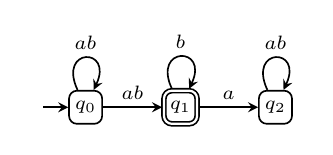
\begin{tikzpicture}[my automaton,semithick]
\scriptsize
\node[state,initial]              (0) {$q_0$};
\node[state,accepting,right=of 0] (1) {$q_1$};
\node[state,,right=of 1]          (2) {$q_2$};
\path[->] (0) edge[my above,loop] node[above] {$ab$} ()
          (0) edge                node[above] {$ab$} (1)
          (1) edge[my above,loop] node[above] {$b$}  ()
          (1) edge                node[above] {$a$}  (2)
          (2) edge[my above,loop] node[above] {$ab$} ();
\end{tikzpicture}\hfill}
\begin{itemize}
  \item Finite state automata running on infinite words ($\omega$-words) $\in \Sigma^\omega$
  \item A word is accepted if it has an accepting run
  \item A run is accepting if it visits an accepting state infinitely often
\end{itemize}
\end{block}
\pause
\begin{block}{Büchi complementation}
The complement of a Büchi automaton $A$ is another Büchi automaton $B$, such that:
\begin{quote}
\ita{$B$ accepts a word if and only if it is not accepted by $A$}
\end{quote}
\end{block}
  
%item Büchi automata

  % {\hfill
  % \begin{tikzpicture}[my automaton]
  % \scriptsize
  % \node[state,initial]              (0) {$q_0$};
  % \node[state,accepting,right=of 0] (1) {$q_1$};
  % \node[state,,right=of 1]          (2) {$q_2$};
  % \path[->] (0) edge[my above,loop] node[above] {$ab$} ()
  %           (0) edge                node[above] {$ab$} (1)
  %           (1) edge[my above,loop] node[above] {$b$}  ()
  %           (1) edge                node[above] {$a$}  (2)
  %           (2) edge[my above,loop] node[above] {$ab$} ();
  % \end{tikzpicture}\hfill}

%   \begin{itemize}
%   \item Finite state automata running on infinite words ($\omega$-words) $\in \Sigma^\omega$
%   \item A word is accepted if it has an accepting run
%   \item A run is accepting if it visits an accepting state infinitely often
%   \end{itemize}
% \item Büchi complementation
%   \begin{itemize}
%   \item Given a Büchi automaton $A$, construct another Büchi automaton $B$
%   \item $\dots$ such that $B$ accepts a word if an only if it is nota accepted by $A$
%   \end{itemize}
% \end{itemize}
\end{frame}

%------------------------------------------------------------------------------%
% Frame
%------------------------------------------------------------------------------%
\begin{frame}{Büchi Complementation Constructions}
%\vspace{-0.1cm} % Modify vertical alignment of image
\centering
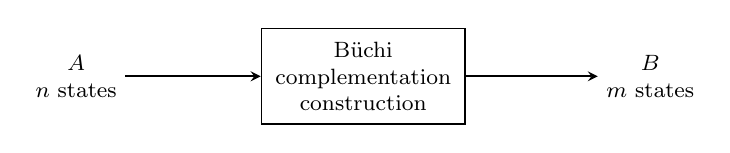
\begin{tikzpicture}[c/.style={align=center},semithick]
\footnotesize
\node (a) [c]                              {$A$\\$n$ states};
\node (b) [c,node distance=6cm,right=of a] {$B$\\$m$ states};
\node (c) at ($(a)!0.5!(b)$) [c,draw,inner sep=5pt]{Büchi\\complementation\\construction};
\draw[->] (a.east) to (c.west);
\draw[->] (c.east) to (b.west);
\end{tikzpicture}
\begin{itemize}
\item Different constructions produce different complements $B$ for the same automaton $A$
\item Main performance measure: number $m$ of states of $B$ in relation to number $n$ of states of $A$
  \begin{itemize}
  \item State complexity
  \item Also known as state growth, state blow-up, or state explosion
  \item E.g. if $n=10$ and $m=100$, then $m=n^2$
  \item Biggest problem of Büchi complementation
  \end{itemize}
\end{itemize}
\end{frame}


%------------------------------------------------------------------------------%
% Frame
%------------------------------------------------------------------------------%
\begin{frame}{The Fribourg Construction}
%\vspace{-0.1cm} % Modify vertical alignment of image
\begin{itemize}
\item Slice-based complementation construction
\item Worst-case state complexity: $(1.59n)^n$
\item Optimisations:
  \begin{itemize}
  \item R2C: if input automaton is complete, remove states whose rightmost component is 2-coloured
  \item M1: merge certain adjacent components ($1.195n)^n$)
  \item M2: keep not more than one 2-coloured component in every state ($0.86n^n$)
  \end{itemize}
\end{itemize}
\end{frame}


\section{GOAL}
%------------------------------------------------------------------------------%
% Frame
%------------------------------------------------------------------------------%
\begin{frame}{GOAL}
%\vspace{-0.1cm} % Modify vertical alignment of image
\begin{itemize}
\item \fat{G}raphical Tool for \fat{O}mega-\fat{A}utomata and \fat{L}ogics
\item \url{http://goal.im.ntu.edu.tw/wiki/doku.php}
\item Create and manipulate $\omega$-automata
\end{itemize}
\centering
\begin{tabular}{cc}
\footnotesize Graphical user interface & \footnotesize Command line interface \\
\includegraphics[width=0.46\textwidth,trim={0 2cm 0 0},clip]
{figures/goal_gui.png} &
\includegraphics[width=0.46\textwidth,trim={0 2cm 0 0},clip]
{figures/goal_cl.png}
\end{tabular}
\end{frame}

%------------------------------------------------------------------------------%
% Frame
%------------------------------------------------------------------------------%
\begin{frame}{GOAL: Büchi Complementation Constructions}
%\vspace{-0.1cm} % Modify vertical alignment of image
\begin{itemize}
\item Implementations of several Büchi complementation constructions (GOAL version 2014--11--17)
\end{itemize}
\centering
\footnotesize
\begin{tabular}{ll}
\hline
GOAL Name & Reference \\
\hline
Ramsey        & \cite{1985_sistla,PrasadSistla1987217} \\
Safra         & \cite{1988_safra_2,1988_safra_1} \\
MS            & \cite{Muller199569} \\
ModifiedSafra & \cite{2006_althoff} \\
Piterman      & \cite{2006_piterman,2007_piterman} \\
WAA           & \cite{1997_vardi,Kupferman:2001} \\
WAPA          & \cite{1999_thomas} \\
Rank          & \cite{schewe2009buchi} \\
Slice+P       & \cite{vardi2007automata} \\
Slice         & \cite{2008_kaehler} \\
\hline
\end{tabular}
\end{frame}

%------------------------------------------------------------------------------%
% Frame
%------------------------------------------------------------------------------%
\begin{frame}{Fribourg Construction Plugin for GOAL}
%\vspace{-0.1cm} % Modify vertical alignment of image
\begin{itemize}
\item GOAL is built with the Java Plugin Framework (JPF)\footnote{\scriptsize\url{http://jpf.sourceforge.net/}}
  \begin{itemize}
  \item Extensibility: create \fat{plugins} containing \fat{extensions} for pre-defined \fat{extension points}
  \end{itemize}
\item Our plugin adds the Fribourg construction to GOAL
  \begin{itemize}
  \item $\dots$ in a fully integrated way
  \end{itemize}
\end{itemize}
\centering
\begin{tabular}{cc}
\footnotesize Graphical user interface & \footnotesize Command line interface \\
\includegraphics[width=0.46\textwidth]{figures/plugin_gui.png} &
\includegraphics[width=0.46\textwidth]{figures/plugin_cl.png}
\end{tabular}
\begin{itemize}
\item Download: \url{https://frico.s3.amazonaws.com/goal_plugins/ch.unifr.goal.complement.zip}
\end{itemize}
\end{frame}

%------------------------------------------------------------------------------%
% Frame
%------------------------------------------------------------------------------%
\begin{frame}{GOAL and Plugin Demo}
\vspace{0.5cm}
\centering
\includegraphics[width=0.9\textwidth]{figures/goal_logo.png}
\end{frame}

%------------------------------------------------------------------------------%
% Frame
%------------------------------------------------------------------------------%
\begin{frame}{Test Data: GOAL Test Set}
\begin{itemize}
\item Created and used for~\cite{2011_tsai}
\item 11,000 automata
  \begin{itemize}
  \item 15 states
  \item Alphabet $\Sigma = \{0, 1\}$
  \item 11 transition densities
    \begin{itemize}
    \item $\mathcal T=(1.0,\,1.2,\,1.4,\,1.6,\,1.8,\,2.0,\,2.2,\,2.4,\,2.6,\,2.8,\,3.0)$
    \end{itemize}
  \item 10 acceptance densities
    \begin{itemize}
    \item $\mathcal A=(0.1,\,0.2,\,0.3,\,0.4,\,0.5,\,0.6,\,0.7,\,0.8,\,0.9,\,1.0)$
    \end{itemize}
  \item 110 classes at 100 automata for each combination of $\mathcal T \times \mathcal A$
  \end{itemize}
\pause
\item Analysis
  \begin{itemize}
  \item 61.8\% universal automata
  \item 0.6\% empty automata
  \item 9.0\% complete automata
  \end{itemize}
\pause
\item Download: \url{https://frico.s3.amazonaws.com/test_sets/goal.zip}
\end{itemize}
\end{frame}

%------------------------------------------------------------------------------%
% Frame
%------------------------------------------------------------------------------%
\newcommand{\Michel}{
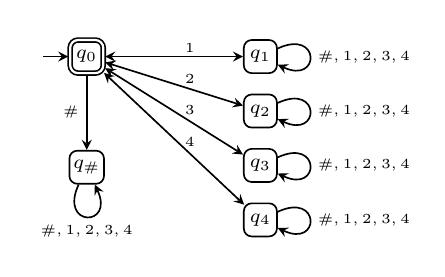
\begin{tikzpicture}[my automaton,semithick]
\scriptsize
% Starting node and # node
\node[state,initial,accepting] (0)               {$q_0$};
\node[state,yshift=-0.2cm]                   (x) [below=of 0]  {$q_\#$};
\draw[->] (0) edge node[left] {\tiny\#} (x);
\draw[->] (x) edge[my below,loop] node[below] {\tiny $\#,1,2,3,4$} ();
% Node 1
\node[state,xshift=1cm]        (1) [right=of 0]  {$q_1$};
\draw[<->] (0) edge node[above,xshift=2mm,yshift=-0.5mm] {\tiny $1$} (1);
\draw[->] (1) edge[my right,loop] node[right] {\tiny $\#,1,2,3,4$} ();
% Node 2
\node[state,yshift=0.5cm]      (2) [below=of 1]  {$q_2$};
\draw[<->] (0) edge node[above,xshift=2mm,yshift=-1mm] {\tiny $2$} (2);
\draw[->] (2) edge[my right,loop] node[right] {\tiny $\#,1,2,3,4$} ();
% Node 3
\node[state,yshift=0.5cm]      (3) [below=of 2]  {$q_3$};
\draw[<->] (0) edge node[above,xshift=2mm,yshift=-1.5mm] {\tiny $3$} (3);
\draw[->] (3) edge[my right,loop] node[right] {\tiny $\#,1,2,3,4$} ();
% Node 4
\node[state,yshift=0.5cm]      (4) [below=of 3]  {$q_4$};
\draw[<->,shorten >=-0.2mm,shorten <=-0.2mm] (0) edge node[above,xshift=2mm,yshift=-2mm] {\tiny $4$} (4);
\draw[->] (4) edge[my right,loop] node[right] {\tiny $\#,1,2,3,4$} ();
\end{tikzpicture}
}

\begin{frame}{Test Data: Michel Test Set}
\begin{itemize}
\item Four Michel automata
  \begin{itemize}
  \item Michel 1: 3 states, 2 symbols, 5 transitions
  \item Michel 2: 4 states, 3 symbols, 8 transitions
  \item Michel 3: 5 states, 4 symbols, 11 transitions
  \item Michel 4: 6 states, 5 symbols, 14 transitions
  \end{itemize}

\centering
{\renewcommand{\tabcolsep}{0cm}
\begin{tabular}{m{1.75cm}m{7cm}}
Michel 4: & \Michel
\end{tabular}}

\pause
\raggedright
\item Automata used by~\cite{michel1988} to prove $n!$ lower bound
\item Very high state complexity
\pause
\item Download: \url{https://frico.s3.amazonaws.com/test_sets/michel.zip}
\end{itemize}
\end{frame}

%------------------------------------------------------------------------------%
% Frame
%------------------------------------------------------------------------------%
% Black dash itemize symbol
\newcommand{\myitem}{\item[\color{black}{--}]}
% Shortcut commands for usage in table
\newcommand{\igoal}{
\begin{itemize}\itemsep0pt
\myitem Fribourg
\myitem Fribourg+R2C
\myitem Fribourg+R2C+C
\myitem Fribourg+M1
\myitem Fribourg+M1+R2C
\myitem Fribourg+M1+R2C+C
\myitem Fribourg+M1+M2
\myitem Fribourg+R
\end{itemize}}

\newcommand{\imichel}{
\begin{itemize}\itemsep0pt
\myitem Fribourg
\myitem Fribourg+R2C
\myitem Fribourg+M1
\myitem Fribourg+M1+M2
\myitem Fribourg+M1+M2+R2C
\myitem Fribourg+R
\end{itemize}}

\newcommand{\egoal}{
\begin{itemize}\itemsep0pt
\myitem Fribourg+M1+R2C
\myitem Piterman+EQ+RO
\myitem Rank+TR+RO
\myitem Slice+P+RO+MADJ+EG
\end{itemize}}

\newcommand{\emichel}{
\begin{itemize}\itemsep0pt
\myitem Fribourg+M1+M2+R2C
\myitem Piterman+EQ+RO
\myitem Rank+TR+RO
\myitem Slice+P+RO+MADJ+EG
\end{itemize}}

\begin{frame}{Test Setup}
\begin{itemize}
\item Internal tests
  \begin{itemize}
  \item Compare different versions of the Fribourg construction
  \end{itemize}
\item External tests
  \begin{itemize}
  \item Compare Fribourg construction with other constructions
  \end{itemize}
\end{itemize}
\pause
\centering
\scriptsize
\begin{tabular}{l|c|c}
& GOAL test set & Michel test set \\
\hline
Internal tests & \parbox{4.25cm}{\igoal} & \raisebox{1.125em}{\parbox{4.25cm}{\imichel}} \\
\hline
External tests & \parbox{4.25cm}{\egoal} & \parbox{4.25cm}{\emichel}
\end{tabular}
\end{frame}

%------------------------------------------------------------------------------%
% Frame
%------------------------------------------------------------------------------%
\begin{frame}{Results: Internal Tests on GOAL Test Set}
\centering
\scriptsize
{\renewcommand{\arraystretch}{1.15}
\input{figures/i.g/table_states.tex}}
\end{frame}

%------------------------------------------------------------------------------%
% Frame
%------------------------------------------------------------------------------%
\begin{frame}{Results: Internal Tests on GOAL Test Set}
\centering
\includegraphics[width=0.9\textwidth]{figures/i.g/strip.pdf}
\end{frame}

%------------------------------------------------------------------------------%
% Frame
%------------------------------------------------------------------------------%
\begin{blank}
\begin{frame}{}
\vspace{0.25cm}
\centering
\footnotesize
{\renewcommand{\tabcolsep}{0cm}
\renewcommand{\arraystretch}{1}
\begin{tabular}{cc}
\includegraphics[width=0.4\textwidth]{figures/i.g/Fribourg.pdf} &
\includegraphics[width=0.4\textwidth]{figures/i.g/Fribourg+R2C.pdf} \\
Fribourg & Fribourg+R2C \\
\includegraphics[width=0.4\textwidth]{figures/i.g/Fribourg+R2C+C.pdf} &
\includegraphics[width=0.4\textwidth]{figures/i.g/Fribourg+R.pdf} \\
Fribourg+R2C+C & Fribourg+R
\end{tabular}}
\end{frame}
\end{blank}

%------------------------------------------------------------------------------%
% Frame
%------------------------------------------------------------------------------%
\begin{blank}
\begin{frame}{}
\vspace{0.25cm}
\centering
\footnotesize
{\renewcommand{\tabcolsep}{0cm}
\renewcommand{\arraystretch}{1}
\begin{tabular}{cc}
\includegraphics[width=0.4\textwidth]{figures/i.g/Fribourg+M1.pdf} &
\includegraphics[width=0.4\textwidth]{figures/i.g/Fribourg+M1+R2C.pdf} \\
Fribourg+M1 & Fribourg+M1+R2C \\
\includegraphics[width=0.4\textwidth]{figures/i.g/Fribourg+M1+R2C+C.pdf} &
\includegraphics[width=0.4\textwidth]{figures/i.g/Fribourg+M1+M2.pdf} \\
Fribourg+M1+R2C+C & Fribourg+M1+M2
\end{tabular}}
\end{frame}
\end{blank}

%------------------------------------------------------------------------------%
% Frame
%------------------------------------------------------------------------------%
\begin{frame}{$ $}
\centering
\tikz \node[rectangle,draw,rounded corners=1mm,fill=blue!20,inner sep=8pt] {Thank you very much for listening!};
\end{frame}

% Following frames are counted separately with the appendixnumberbeamer package
\appendix
%------------------------------------------------------------------------------%
% References
%------------------------------------------------------------------------------%
\begin{frame}[t,allowframebreaks]{References}
%\nocite{*} % If active, display all bib entries, and not just the cited ones
\bibliographystyle{apalike}
{\tiny
\bibliography{../bib/buchi_compl.bib}}
\end{frame}


\end{document}
